\documentclass{article}
\usepackage[english]{babel}
\usepackage{amsmath}
\usepackage{amssymb}
\usepackage{amsthm}
\usepackage{amsfonts}
\usepackage{blindtext}
\usepackage{systeme}
\usepackage{relsize}
\usepackage{enumerate}
\usepackage{commath}
\usepackage{mathrsfs}
\usepackage{bm}
\usepackage{graphicx}
\usepackage{wrapfig}
\usepackage{subcaption}
\usepackage{tikz-cd}
\usetikzlibrary{automata,positioning}
%\usepackage{hyperref}
%\hypersetup{
% colorlinks=false,% hyperlinks will be black
%linkbordercolor=black,% hyperlink borders will be red
%pdfborderstyle={/S/U/W 0.25}% border style will be underline of width 1pt
%}
\usepackage{chngcntr}
\usepackage{MnSymbol}
\usepackage{tikz}
\usepackage[margin=0.75in]{geometry}
\usepackage{cleveref}

\newcommand{\C}{\mathbf{C}}
\newcommand{\R}{\mathbf{R}}
\newcommand{\Q}{\mathbf{Q}}
\newcommand{\Z}{\mathbf{Z}}
\newcommand{\N}{\mathbf{N}}
\newcommand{\E}{\mathbf{E}}
\newcommand{\B}{\mathbf{B}}
\newcommand{\F}{\mathbf{F}}
\newcommand{\U}{\mathbf{U}}
\newcommand{\V}{\mathbf{V}}
\newcommand{\J}{\mathbf{J}}
\newcommand{\x}{\mathbf{x}}
\newcommand{\y}{\mathbf{y}}
\newcommand{\z}{\mathbf{z}}
\newcommand{\Sb}{\mathbf{S}}
\newcommand{\Cs}{\mathscr{C}}
\newcommand{\As}{\mathscr{A}}
\newcommand{\I}{\textnormal{\textbf{I}}}
\newcommand{\Id}{\dot{\textnormal{\textbf{I}}}}
\newcommand{\Top}{\textnormal{\textbf{Top}}}
\newcommand{\hTop}{\textnormal{\textbf{hTop}}}
\newcommand{\Groups}{\textnormal{\textbf{Groups}}}
\newcommand{\Set}{\textnormal{\textbf{Set}}}
\newcommand{\Xib}{\mathbf{\Xi}}
\newcommand{\Sym}{\text{Sym}}
\newcommand{\prid}[1]{\langle #1 \rangle}
\newcommand{\apoly}[1]{a_{#1} + a_{#1}x+ a_{#1}x^2 + \cdots + a_{#1}x^n}
\newcommand{\dist}{\textnormal{dist}}
\newcommand{\ti}[1]{\textit{#1}}
\newcommand{\tb}[1]{\textnormal{\textbf{#1}}}
\newcommand{\es}{\emptyset}
\newcommand{\sst}{\subset}
\newcommand{\ssteq}{\subseteq}
\newcommand{\func}[3]{#1: #2 \to #3}
\newcommand{\inte}[1]{\textnormal{int}(#1)}
\newcommand{\bdr}[1]{\textnormal{bdry}(#1)}
\newcommand{\ifff}{if and only if }
\newcommand{\st}{such that }
\newcommand{\wrt}{with respect to }
\newcommand{\tspace}[1]{\text{T}_#1}
\newcommand{\mathdash}{\hbox{-}}
\newcommand{\diam}[1]{\textnormal{diam}(#1)}
\newcommand{\setst}{\hspace{1mm} | \hspace{1mm} }
\newcommand{\supp}{\textnormal{support}}
\newcommand{\clos}{\textnormal{closure}}
\newcommand{\rel}{\textnormal{rel }}
\newcommand{\Hom}{\textnormal{Hom}}
\newcommand{\obj}{\textnormal{obj}}
\newcommand{\varlisto}[2]{#1_1,#1_2,\ldots,#1_{#2}}
\newcommand{\varlistz}[2]{#1_0,#1_1,\ldots,#1_{#2}}
\newcommand{\finv}[2]{#1^{-1}(#2)}
\newcommand{\disu}{\rotatebox[origin=c]{90}{$\models$}}
\newcommand{\rank}{\textnormal{rank }}
\newcommand{\card}{\textnormal{card }}
\newcommand{\im}{\textnormal{im }}
\newcommand{\cls}{\textnormal{cls }}
\newcommand{\rev}{\textnormal{rev }}
\newcommand{\defeq}{\mathrel{\stackrel{\makebox[0pt]{\mbox{\normalfont\tiny def}}}{=}}}



%\renewcommand{\phi}{\varphi}
\renewcommand{\epsilon}{\varepsilon}


\newtheorem{theorem}{Theorem}[section]
\newtheorem{corollary}[theorem]{Corollary}
\newtheorem{proposition}{Proposition}[theorem]
\newtheorem{lemma}[theorem]{Lemma}
\theoremstyle{definition}
\newtheorem*{definition}{Definition}
\newtheorem*{remark}{Remark}
\newtheorem*{remarks}{Remarks}


\renewcommand\qedsymbol{$\blacksquare$}
\setcounter{section}{-1}

\counterwithin*{equation}{section}

\title{CSCI 3434 Theory of Computation Homework 1}
\author{Luke Meszar (Worked with Jeff Lipnick)}
\date{September 13, 2017}
\begin{document}
\maketitle
\begin{enumerate}
	\item[HW 1.1] Design deterministic finite automata for each of the following sets:
	\begin{enumerate}
		\item the set of strings in $\{4,8,1\}^*$ containing the substring 481;
		
		Consider the following DFA:
		
		\begin{center}
			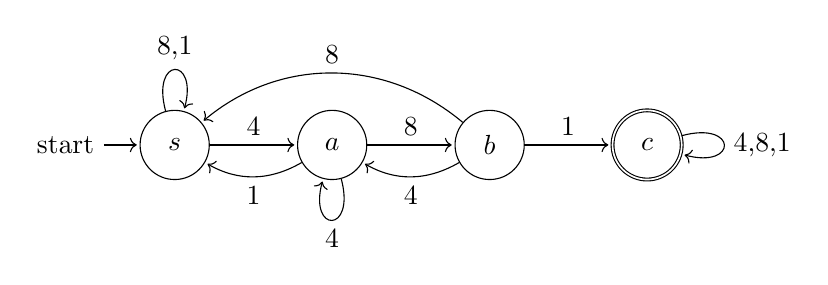
\begin{tikzpicture}[shorten >=1pt,node distance=2cm,on grid,auto]
			\node[state,initial](s) {$s$};
			\node[state](a)[right=of s] {$a$};
			\node[state](b)[right=of a] {$b$};
			\node[state,accepting](c)[right=of b] {$c$};
			\path[->]
			(s) edge node {4} (a)
			(a) edge node {8} (b)
			(b) edge node {1} (c)
			(s) edge [loop above] node {8,1} ()
			(a) edge [bend left] node {1} (s)
			(b) edge [bend right=40,swap] node {8} (s)
			(c) edge [loop right] node {4,8,1} ()
			(a) edge [loop below] node {4} ()
			(b) edge [bend left] node {4} (a);
			\end{tikzpicture}
		\end{center}
	
		At the first state, the DFA can only from state $s$ if there is a four in the string. Otherwise, it continues looping at state $s$ until it sees a 4 meaning it can begin looking for $481$. Then, in state $a$, it can only continue onwards to state $b$ if it sees an $8$. Otherwise, if it sees a 1, then it has to go back to the state $s$; but if it sees a four, it should stay at state $a$ so it can check for an 8 again. Then, at state $b$, it continues onto state $c$ if it sees a 1, because it has found the substring 481. If it sees an 8, then it has to go back to $s$ so it can start the search over. If it sees a 4, then it only has to go back to $a$ since state $a$ is the state representing, ``I have seen a 4'' already. Once the DFA reaches state $c$, then it loops there till the end of the string since it has already found the substring 481 and it doesn't care what comes afterwards.  
		\item the set of strings in $\{a\}^*$ whose length is divisible by either 2 or 7;
		
		Consider the DFA $M_1$ that accepts strings in $\{a\}^*$ with length divisible by 2:
		\begin{center}
			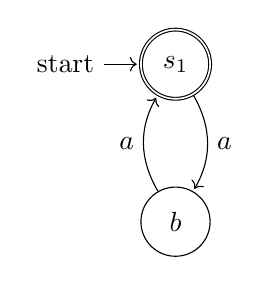
\begin{tikzpicture}[shorten >=1pt,node distance=2cm,on grid,auto]
			\node[state,initial,accepting](s1) {$s_1$};
			\node[state](b)[below=of s1] {$b$};
			\path[->]
			(s1) edge [bend left] node {$a$} (b)
			(b) edge [bend left] node {$a$} (s1);
			\end{tikzpicture}
		\end{center}
	
		$M_1$ works by counting the number of $a$'s mod 2. It accepts every second $a$ so if the string has even length, then it will end in the accept state, $s_1$. 
		
		Also consider the DFA $M_2$ that accepts strings in $\{a\}^*$ with length divisible by 7
		\begin{center}
			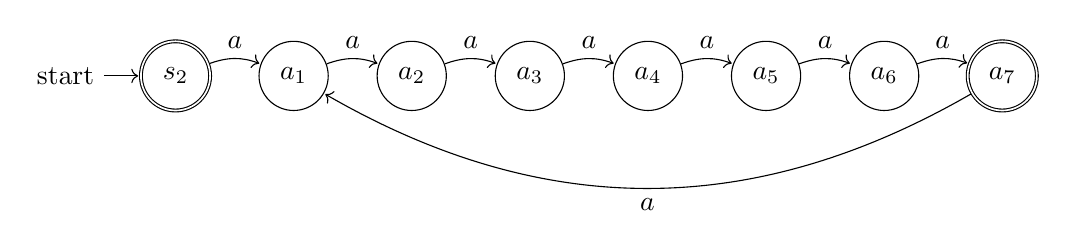
\begin{tikzpicture}[shorten >=0.5pt,node distance=1.5cm,on grid,auto]
			\node[state,initial,accepting](s2) {$s_2$};
			\node[state](a1)[right=of s2] {$a_1$};
			\node[state](a2)[right=of a1] {$a_2$};
			\node[state](a3)[right=of a2] {$a_3$};
			\node[state](a4)[right=of a3] {$a_4$};
			\node[state](a5)[right=of a4] {$a_5$};
			\node[state](a6)[right=of a5] {$a_6$};
			\node[state,accepting](a7)[right=of a6] {$a_7$};
			\path[->]
			(s2) edge [bend left=20] node {$a$} (a1)
			(a1) edge [bend left=20] node {$a$} (a2)
			(a2) edge [bend left=20] node {$a$} (a3)
			(a3) edge [bend left=20] node {$a$} (a4)
			(a4) edge [bend left=20] node {$a$} (a5)
			(a5) edge [bend left=20] node {$a$} (a6)
			(a6) edge [bend left=20] node {$a$} (a7)
			(a7) edge [bend left] node {$a$} (a1);
			\end{tikzpicture}
		\end{center}
		$M_2$ works by counting the number of $a$'s mod 7. From the start, $s_2$, it moves forward 7 states and then accepts. It is important that from $a_7$, the DFA transitions to $a_1$. If it instead went back to $s_2$, then on every subsequent loop through $M_2$, it would be string whose length were of the form $7 + 8k$ for $k \in \N$. By going from $a_7$ to $a_1$, it only counts 7 $a$'s on successive loops through the automaton. 
	
		Then using the product construction for unions, we get:
		\begin{center}
			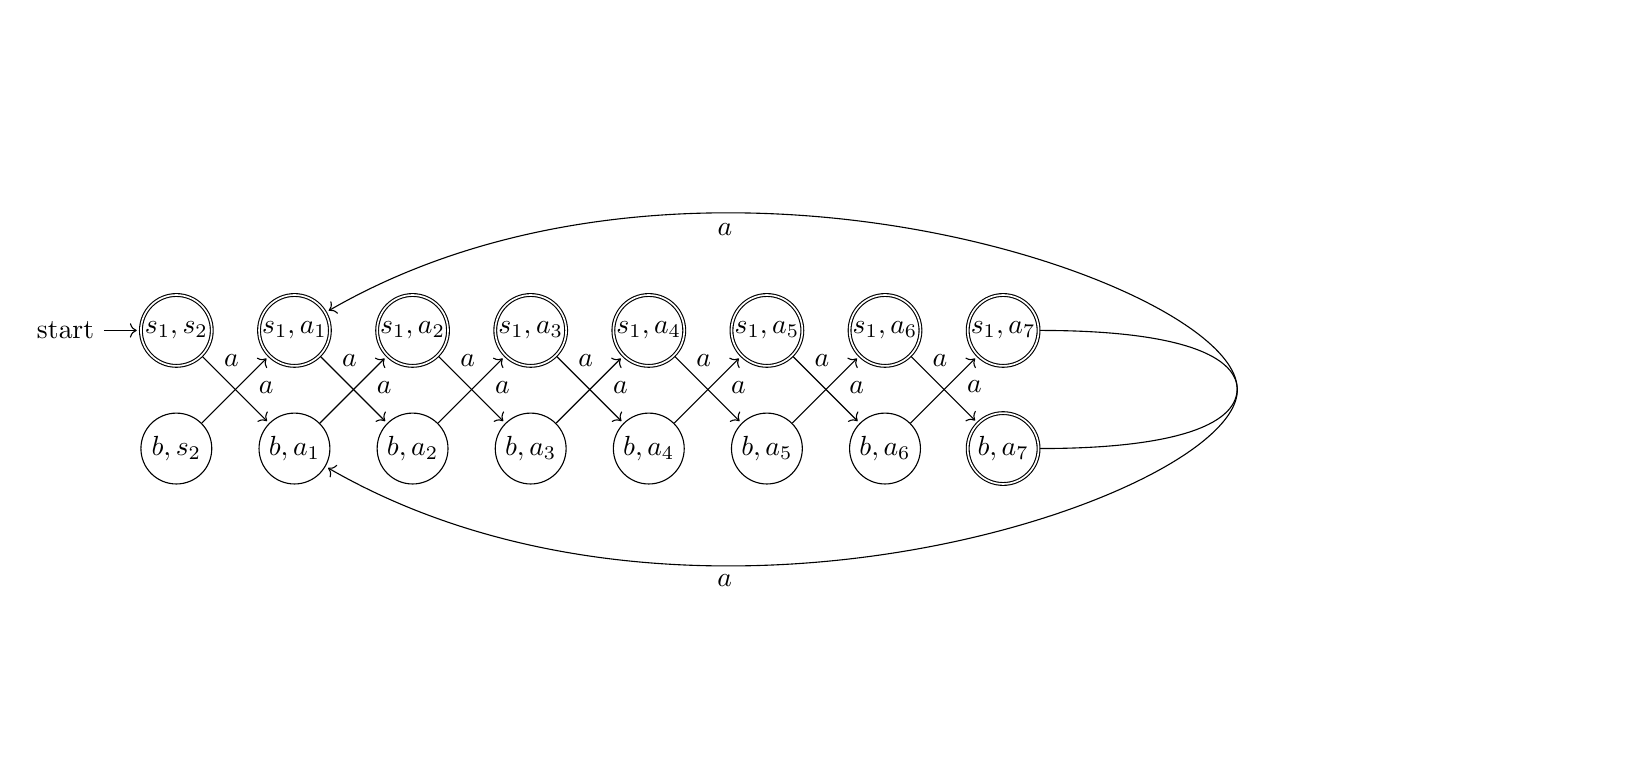
\begin{tikzpicture}[shorten >=1pt,node distance=1.5cm,on grid,auto]
			\node[state,initial,accepting,inner sep=0pt,minimum size=0.9cm](s1s2) {$s_1,s_2$};
			\node[state,accepting,inner sep=0pt,minimum size=0.9cm](s1a1)[right=of s1s2] {$s_1,a_1$};
			\node[state,accepting,inner sep=0pt,minimum size=0.9cm](s1a2)[right=of s1a1] {$s_1,a_2$};
			\node[state,accepting,inner sep=0pt,minimum size=0.9cm](s1a3)[right=of s1a2] {$s_1,a_3$};
			\node[state,accepting,inner sep=0pt,minimum size=0.9cm](s1a4)[right=of s1a3] {$s_1,a_4$};
			\node[state,accepting,inner sep=0pt,minimum size=0.9cm](s1a5)[right=of s1a4] {$s_1,a_5$};
			\node[state,accepting,inner sep=0pt,minimum size=0.9cm](s1a6)[right=of s1a5] {$s_1,a_6$};
			\node[state,accepting,inner sep=0pt,minimum size=0.9cm](s1a7)[right=of s1a6] {$s_1,a_7$};
			\node[state,inner sep=0pt,minimum size=0.9cm](bs2)[below=of s1s2] {$b,s_2$};
			\node[state,inner sep=0pt,minimum size=0.9cm](ba1)[below=of s1a1] {$b,a_1$};
			\node[state,inner sep=0pt,minimum size=0.9cm](ba2)[below=of s1a2] {$b,a_2$};
			\node[state,inner sep=0pt,minimum size=0.9cm](ba3)[below=of s1a3] {$b,a_3$};
			\node[state,inner sep=0pt,minimum size=0.9cm](ba4)[below=of s1a4] {$b,a_4$};
			\node[state,inner sep=0pt,minimum size=0.9cm](ba5)[below=of s1a5] {$b,a_5$};
			\node[state,inner sep=0pt,minimum size=0.9cm](ba6)[below=of s1a6] {$b,a_6$};
			\node[state,accepting, inner sep=0pt,minimum size=0.9cm](ba7)[below=of s1a7] {$b,a_7$};
			\path[->]
			(s1s2) edge node [pos=0.7] {$a$} (ba1)
			(s1a1) edge node [pos=0.7] {$a$} (ba2)
			(s1a2) edge node [pos=0.7] {$a$} (ba3)
			(s1a3) edge node [pos=0.7] {$a$} (ba4)
			(s1a4) edge node [pos=0.7] {$a$} (ba5)
			(s1a5) edge node [pos=0.7]  {$a$} (ba6)
			(s1a6) edge node [pos=0.7] {$a$} (ba7)
			(s1a7) edge [out=0,in=330,looseness=2] node [pos=0.75] {$a$} (ba1)
			(bs2) edge node [pos=0.7] {$a$} (s1a1)
			(ba1) edge node [pos=0.7] {$a$} (s1a2)
			(ba2) edge node [pos=0.7] {$a$} (s1a3)
			(ba3) edge node [pos=0.7] {$a$} (s1a4)
			(ba4) edge node [pos=0.7] {$a$} (s1a5)
			(ba5) edge node [pos=0.7] {$a$} (s1a6)
			(ba6) edge node [pos=0.7] {$a$} (s1a7)
			(ba7) edge [out=0,in=30 ,looseness=2] node [pos=0.75]  {$a$} (s1a1);
			\end{tikzpicture}
		\end{center}
	
		This DFA has states corresponding to the Cartesian product of the states of $M_1$ and $M_2$. The transition function is defined based on where each state in the pair went to on a given input in their original machines. The final states consist of any state in which one of the elements in the Cartesian product was a final state in either $M_1$ or $M_2$.
		\item the set of strings $x \in \{0,1\}^*$ such that $\#0(x)$ is even and $\#1(x)$ is a multiple of three.
		
		Let $M_1$ be the DFA that accepts strings $x \in \{0,1\}^*$ such that $\#0(x)$ is even. 
		\begin{center}
			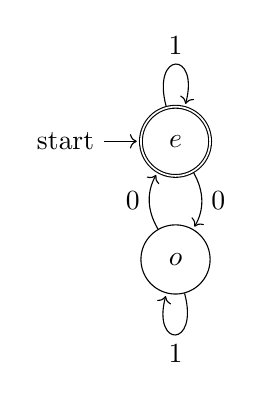
\begin{tikzpicture}[shorten >=1pt,node distance=1.5cm,on grid,auto]
			\node[state,initial,accepting](e) {$e$};
			\node[state](o)[below=of e] {$o$};
			\path[->]
			(e) edge [bend left] node {0} (o)
			(o) edge [bend left] node {0} (e)
			(e) edge [loop above] node {1} ()
			(o) edge [loop below] node {1} ();
			\end{tikzpicture}
		\end{center}
	
	This DFA works very similarly to the first one in the previous problem. The only difference is that it doesn't let the number of 1's affect the result so it doesn't change states when it sees a 1, only when it sees a zero.
	Then, let $M_2$ be the DFA that accepts strings  $x \in \{0,1\}^*$ such that $\#1(x)$ is a multiple of 3. 
	\begin{center}
		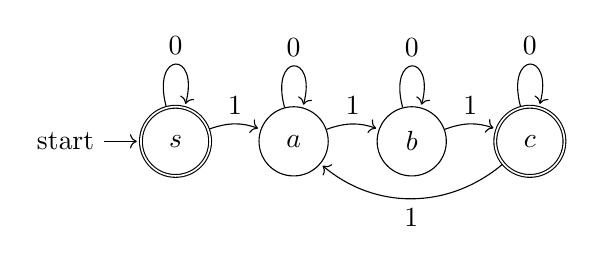
\begin{tikzpicture}[shorten >=1pt,node distance=1.5cm,on grid,auto]
		\node[state,initial,accepting](s) {$s$};
		\node[state](a)[right=of s] {$a$};
		\node[state](b)[right=of a] {$b$};
		\node[state,accepting](c)[right=of b] {$c$};
		\path[->]
		(s) edge [bend left=20] node {1} (a)
		(a) edge [bend left=20] node {1} (b)
		(b) edge [bend left=20] node {1} (c)
		(c) edge [bend left=40] node {1} (a)
		(s) edge [loop above] node {0} ()
		(a) edge [loop above] node {0} ()
		(b) edge [loop above] node {0} ()
		(c) edge [loop above] node {0} ();
		\end{tikzpicture}
	\end{center}
	This DFA works very similarly to the second one in the previous problem. Again, the only difference is that it doesn't want the number of 0's to affect the result so it doesn't change states when it sees a 0, only when it sees a 1. 

	Then using the product construction for intersections, we get
	\begin{center}
		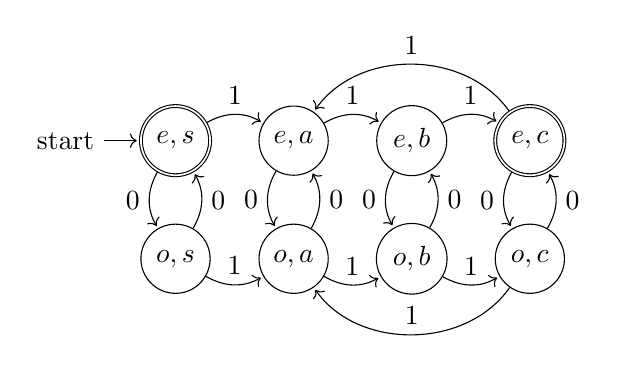
\begin{tikzpicture}[shorten >=1pt,node distance=1.5cm,on grid,auto]
		\node[state,initial,accepting](es) {$e,s$};
		\node[state](ea)[right=of es] {$e,a$};
		\node[state](eb)[right=of ea] {$e,b$};
		\node[state,accepting](ec)[right=of eb] {$e,c$};
		\node[state](os)[below=of es] {$o,s$};
		\node[state](oa)[below=of ea] {$o,a$};
		\node[state](ob)[below=of eb] {$o,b$};
		\node[state](oc)[below=of ec] {$o,c$};
		\path[->]
		(es) edge [bend right,swap] node {0} (os)
		(ea) edge [bend right,swap] node {0} (oa)
		(eb) edge [bend right,swap] node {0} (ob)
		(ec) edge [bend right,swap] node {0} (oc)
		(os) edge [bend right,swap] node {0} (es)
		(oa) edge [bend right,swap] node {0} (ea)
		(ob) edge [bend right,swap] node {0} (eb)
		(oc) edge [bend right,swap] node {0} (ec)
		(es) edge [bend left] node {1} (ea)
		(ea) edge [bend left] node {1} (eb)
		(eb) edge [bend left] node {1} (ec)
		(os) edge [bend right] node {1} (oa)
		(oa) edge [bend right] node {1} (ob)
		(ob) edge [bend right] node {1} (oc)
		(ec) edge [bend right=55,swap] node {1} (ea)
		(oc) edge [bend left=55,swap] node {1} (oa);
		\end{tikzpicture}
	\end{center}

	Here, the states are the Cartesian product of the states of $M_1$ and $M_2$. The transition function is defined based on where each state in the pair went to on a given input in their original machines. The final state is the one where both elements in the ordered pair of the Cartesian product were finals states in their respective machines. In this case, that is the state $(e,c)$ since state $e$ was the final state in $M_1$ and state $c$ was the final state in $M_2$.m 
	\end{enumerate}
\item[HW 1.2] Consider the following two deterministic finite automata.
\\
\begin{center}
	\begin{tabular}{cccc}
		& & a & b \\\cline{3-4}
		$\rightarrow$ & \multicolumn{1}{c|}{1} & 1 & 2\\
		& \multicolumn{1}{c|}{2F} & 2 & 1\\
	\end{tabular}
	\hspace{4cm}
	\begin{tabular}{cccc}
		& & a & b \\\cline{3-4}
		$\rightarrow$ & \multicolumn{1}{c|}{1} &2 & 3\\
		& \multicolumn{1}{c|}{2} & 3 & 1\\
		& \multicolumn{1}{c|}{3F} & 1 & 2\\
	\end{tabular}
\end{center}


Use the product construction to produce deterministic automata accepting (a) the intersection and (b) the union of the two sets accepted by these automata.

For the intersection, we use the product construction. The final state is the ordered pair where both elements are final states in their respective machines. In this example, this  corresponds to (2,3). 
\begin{center}
	\begin{tabular}{cccc}
		& & a & b \\\cline{3-4}
		$\rightarrow$ & \multicolumn{1}{l|}{(1,1)} & (1,2) & (2,3) \\
		& \multicolumn{1}{l|}{(1,2)} & (1,3) & (2,1) \\
		& \multicolumn{1}{l|}{(1,3)} & (1,1) & (2,2) \\
		& \multicolumn{1}{l|}{(2,1)} & (2,2) & (1,3) \\
		& \multicolumn{1}{l|}{(2,2)} & (2,3) & (1,1) \\
		& \multicolumn{1}{l|}{(2,3)F} & (2,1) & (1,2) \\
	\end{tabular}
\end{center}

For the union, we use the product construction. The final states are the ordered pairs where at least on of the elements in a final state in its respective machine. In this example, such states are (1,3), (2,1), (2,2), and (2,3). 

\begin{center}
	\begin{tabular}{cccc}
		& & a & b \\\cline{3-4}
		$\rightarrow$ & \multicolumn{1}{l|}{(1,1)} & (1,2) & (2,3) \\
		& \multicolumn{1}{l|}{(1,2)} & (1,3) & (2,1) \\
		& \multicolumn{1}{l|}{(1,3)F} & (1,1) & (2,2) \\
		& \multicolumn{1}{l|}{(2,1)F} & (2,2) & (1,3) \\
		& \multicolumn{1}{l|}{(2,2)F} & (2,3) & (1,1) \\
		& \multicolumn{1}{l|}{(2,3)F} & (2,1) & (1,2) \\
	\end{tabular}
\end{center}
\item[HW 1.3] Let $M = (Q,\Sigma,\delta,s,F)$ be an arbitrary DFA. Prove by induction on $|y|$ that for all strings $x,y \in \Sigma^*$ and $q \in Q$,
\[\hat{\delta}(q,xy) =\hat{\delta}(\hat{\delta}(q,x),y),\]
where $\hat{\delta}$ is the extended version of $\delta$ defined on all strings described in Lecture 3.

\begin{proof}
	Base Case: Let $|y| = 0$ which implies $y = \epsilon$. Then, on the left hand side we get
	\[\hat{\delta}(q,x\epsilon) = \delta(\hat{\delta}(q,x),\epsilon) =\hat{\delta}(q,x)\]
	by the definition of $\hat{\delta}(q,xa)$ and the definition of $\delta(q,\epsilon)$. On the right hand side we get
	\[\hat{\delta}(\hat{\delta}(q,x),\epsilon) = \hat{\delta}(q,x)\]
	by the definition of $\hat{\delta}(q,\epsilon)$. Since the left and right hand sides agree, the base case holds.
	
	Induction Step: Assume $|y| = k$ for some $k \in \N$ and that $\hat{\delta}(q,xy) =\hat{\delta}(\hat{\delta}(q,x),y)$. Now, consider $ya$, a string of length $k + 1$. Then we get:
	\begin{align*}
	\hat{\delta}(q,xya) &= \delta(\hat{\delta}(q,xy),a) \\
	&= \delta(\hat{\delta}(\hat{\delta}(q,x),y),a) \text{ by the induction hypothesis} \\
	&= \hat{\delta}(\hat{\delta}(\hat{\delta}(q,x),y),a) \text{ since } \delta \text{ and } \hat{\delta} \text{ are equivalent for a single symbol} \\
	&= \hat{\delta}(\hat{\delta}(q,x),ya).
	\end{align*}
	Thus, we have shown by induction that $\hat{\delta}(q,xy) =\hat{\delta}(\hat{\delta}(q,x),y)$ for all $x,y \in \Sigma^*$ and $q \in Q$. 
\end{proof}
\item[ME 3] Consider the following nondeterministic finite automaton.\\
\begin{center}
	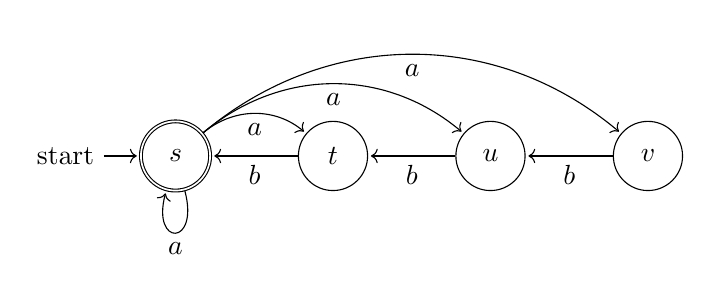
\begin{tikzpicture}[shorten >=1pt,node distance=2cm,on grid,auto]
	\node[state,initial,accepting](q0) {$s$};
	\node[state](q1)[right=of q0] {$t$};
	\node[state](q2)[right=of q1] {$u$};
	\node[state](q3)[right=of q2] {$v$};
	\path[->]
	(q1) edge node {$b$} (q0)
	(q2) edge node {$b$} (q1)
	(q3) edge node {$b$} (q2)
	(q0) edge [loop below] node {$a$} ()
	(q0) edge [bend left=40,swap] node [pos=0.5] {$a$} (q1)
	(q0) edge [bend left=40, swap] node {$a$} (q2)
	(q0) edge [bend left=40,swap] node {$a$} (q3);
	\end{tikzpicture}
\end{center}
\begin{enumerate}
	\item Give a string beginning with $a$ that is \ti{not} accepted.
	
	The string $abbbb$ will not be accepted. The ``closest'' it can get to being accepted is if it takes the path 
	\begin{center}
		\begin{tikzcd}[row sep=small, column sep=small]
			s \arrow[rr, "a"] &  & v \arrow[rr, "b"] &  & u \arrow[rr, "b"] &  & t \arrow[rr, "b"] &  & s \arrow[rr, "b"] &  & \varnothing.
		\end{tikzcd}
	\end{center}
	Any other possible path will end in the empty set even sooner. Any string of the form $ab^n$ for $n \geq 4$ will not be accepted. 
	\item Construct an equivalent deterministic finite automaton using the subset construction. Assuming the states are names $s,t,u,v$ from left to right, show clearly which subset of $\{s,t,u,v\}$ corresponds to each state of the deterministic automaton. Omit inaccessible states. 
	
	Using the subset construction, we get
	\begin{center}
		\begin{tabular}{cccc}
			& & a & b \\\cline{3-4}
			$\rightarrow$ & \multicolumn{1}{r|}{$s$ F} & $stuv$ & $d$\\
			& \multicolumn{1}{r|}{$stuv$ F} & $stuv$ & $stu$ \\
			& \multicolumn{1}{r|}{$stu$ F} & $stuv$ & $st$ \\
			& \multicolumn{1}{r|}{$st$ F} & $stuv$ & $s$ \\
			& \multicolumn{1}{r|}{$d$} & $d$ & $d$ \\
		\end{tabular}
	\end{center}
\end{enumerate}
\item[HW 2.2] The \ti{reverse} of a string $x$, denoted $\rev x$, is $x$ written backwards. Formally,
\[\rev \epsilon \defeq \epsilon, \quad \rev xa \defeq a\ \rev x.\]
For example, $\rev bbaaab = baaabba$. For $A \ssteq \Sigma^*$, define
\[\rev A \defeq \{\rev x \setst x \in A \}.\]
For example, $\rev \{a,ab,aab,aaab\} =\{a,ba,baa,baaa\}$. Show that for any $A \ssteq \Sigma^*$, if $A$ is regular, then so is $\rev A$. 

\begin{proof}
	Assume that $M = (Q,\Sigma,\delta,s,F)$ is a DFA that accepts $A$. Now, construct the following NFA $N = (Q \cup \{q_s\}, \Sigma,\Delta,q_s,s)$. We add a state $q_s$ so that we can treat $M$ as having only one final state. We accomplish this by adding $\epsilon$ transitions between $q_s$ and all $f \in F$. The state $q_s$ becomes our new start state and we will $s$, the start state in $M$ be the final state of $N$. The key construct is the way $\Delta$ is defined. It is defined to reverse the direction of all the arrows in $M$. This is done in the following manner:
	\[\Delta(q,a) = \delta^{-1}(\{q\},a)\]
	where $\delta^{-1}(\{q\},a)$ is the set of all states $r$ such that $\delta(r,a) = q$. We need to make the stipulation that $\Delta(s,a) = s$ for all $a \in \Sigma$. To show that this NFA accepts $\rev A$, we need to show that
	\[\{x \in \Sigma^* \setst \hat{\Delta}(q_s,x) = s\} = \rev A.\]
	
	Denote $\{x \in \Sigma^* \setst \hat{\Delta}(q_s,x) = s\}$ as $\Gamma$.
	We begin by showing that if $x \in \rev A$, then $\hat{\Delta}(q_s,x) = s$. Since $x \in \rev A$, then $\rev x \in A$. This means that there is some sequence of states in $M$
	\begin{center}
		\begin{tikzcd}[row sep=small, column sep=small]
			s \arrow[rr, "a_1"] &  & q_1 \arrow[rr, "a_2"] &  & q_2 \arrow[rr] &  & \cdots \arrow[rr] &  & q_{n} \arrow[rr, "a_{n+1}"] &  & f_i
		\end{tikzcd}
	\end{center}
since $\rev x$ is accepted by $M$. Note that $x = a_{n+1}a_{n}\cdots a_2a_1$. At the beginning, $\Delta(q_s,x)$ $\epsilon$-transitions to all the final states nondeterministically, including $f_i$. Now, $q_n \in \hat{\Delta}(q_s,a_{n+1})$ since $\delta(q_n,a_{n+1}) = f_i$ and $f_i$ is essentially the start state. This is the base case on induction that $\Delta$ maps backwards on this sequence of states. 

Now, for some $k + 1 \in \{1,\ldots,n\}$, assume $q_{k} \in \hat{\Delta}(q_s,a_{n+1}a_{n}\cdots a_{k+1})$. 

Now, we need to show that $q_{k-1} \in \hat{\Delta}(q_s,a_{n+1}a_{n}\cdots a_{k})$. This is equivalent to showing that
\[q_{k-1} \in \bigcup_{q \in D}\Delta(q,a_k)\]
where $D = \hat{\Delta}(q_s,a_{n+1}a_{n}\cdots a_{k+1})$. Well, by our assumption, $q_k \in D$ so we can consider $\Delta(q_k,a_k)$. Well, $q_{k-1} \in \delta^{-1}(q_k,a_k)$ since we know $\delta(q_{k-1},a_k) = q_k$ because $\rev x \in A$. Thus, $q_{k-1} \in \hat{\Delta}(q_s,a_{n+1}a_{n}\cdots a_{k})$. This induction process stops when we get to $k = 1$ and we have $q_1 \in \hat{\Delta}(q_s,a_{n+1}a_{n}\cdots a_{2})$.  To show that $s \in \hat{\Delta}(q_s,a_{n+1}a_{n}\cdots a_{1})$, we just note that this is equivalent to
\[s \in  \bigcup_{q \in D'}\Delta(q,a_1)\]
where $D' = \hat{\Delta}(q_s,a_{n+1}a_{n}\cdots a_{1})$. Well, $q_1 \in D'$ so we can consider $\Delta(q_1,a_1)$. We know that $s \in \delta^{-1}(q_1,a_1)$ since we know $\delta(s,a_1) = q_1$ because $\rev x \in A$. Thus, we have shown that if $x \in \rev A$, then $x \in \Gamma$ so $\rev A \ssteq \Gamma$. 

Now, let $x \in\Gamma$. We want to show that $x \in \rev A$. Since $x \in \Gamma$, there must be some path that is chosen nondeterministically of the following form:
\begin{center}
	\begin{tikzcd}[row sep=small, column sep=small]
		s &  & q_1 \arrow[ll, "a_1"'] &  & q_2 \arrow[ll, "a_2"'] &  & \cdots \arrow[ll] &  & q_n \arrow[ll] &  & f_i \arrow[ll, "a_{n+1}"'].
	\end{tikzcd}
\end{center}
If we can show that $\rev x \in A$, then we know that $x \in \rev A$. To do this, we want to show that $\hat{\delta}(s,\rev x) = \hat{\delta}(s,a_1a_2\cdots a_{n+1}) = f_i$. We begin by proving the base case of 
\[\hat{\delta}(s,a_1) = q_1.\]
Well, we know that $\hat{\delta}(s,a_1) = \delta(s,a_1)$. Then, from the sequence above, we know that $s \in \Delta(q_1,a_1) $ which implies $s \in \delta^{-1}(q_1,a_1)$ which means that $\delta(s,a_1) = q_1$. Thus 
\[\hat{\delta}(s,a_1) = q_1.\]

Next, for some $k \in \{1,\ldots,n\}$ assume that  $\hat{\delta}(s,a_1a_2\cdots a_k) = q_k$. Now consider
\[\hat{\delta}(s,a_1a_2\cdots a_{k+1}) = \delta(\hat{\delta}(s,a_1a_2\cdots a_k),a_{k+1}) = \delta(q_k,a_{k+1}).\]

Then, from the sequence above, we know that $q_k \in \Delta(q_{k+1},a_{k+1})$ which implies $q_{k} \in \delta^{-1}(q_{k+1},a_{k+1})$ which means that $\delta(q_k,a_{k+1}) = q_{k+1}$. Thus 
\[\hat{\delta}(s,a_1a_2\cdots a_{k+1}) = q_k+1.\]
This completes the induction. The inductions stops when we reach the state $q_n$. Then, to show that $\delta(q_n,a_{n+1}) = f_i$, we use the same logic that we have used above about $\Delta(f_i,a_{n+1})$. Thus, $\hat{\delta}(s,\rev x) = f_i$ which implies that $\rev x \in A$ so $x \in \rev A$. This completes the proof that if $A$ is regular, then $\rev A$ is regular. 
\end{proof}
\item[ME 6] Prove that NFAs are exponentially more succinct than DFAS: for any $m$, there exists an NFA with $m$ states such that any equivalent DFA has at least $2^{m-1}$ states.

\begin{proof}
	Let $A_{m+1}$ be the following language:
	\[\{x \in \{0,1\}^* \setst \text{ the } m^{\text{th}} \text{ symbol from the right is a } 1 \}.\]
	An NFA that accepts this language will look like:
	\begin{center}
		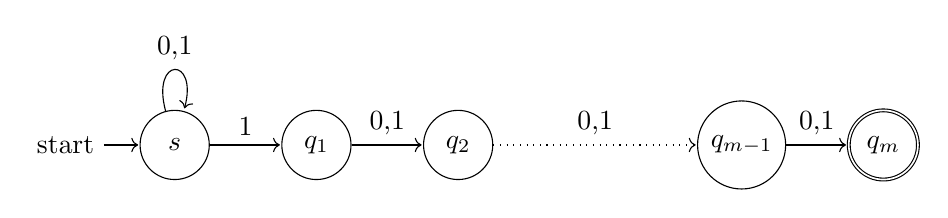
\begin{tikzpicture}[shorten >=0.5pt,node distance=1.8cm,on grid,auto]
		\node[state,initial](s) {$s$};
		\node[state](q1)[right=of s] {$q_1$};
		\node[state](q2)[right=of q1] {$q_2$};
		\node[state,draw=none](em)[right=of q2] {};
		\node[state](qm1)[right=of em] {$\small{q_{m-1}}$};
		\node[state,accepting](qm)[right=of qm1] {$q_m$};
		\path[->]
		(s) edge [loop above] node {0,1} (s)
		(s) edge node {1} (q1)
		(q1) edge node {0,1} (q2)
		(q2) edge [dotted] node {0,1} (qm1)
		(qm1) edge node {0,1} (qm);
		\end{tikzpicture}
	\end{center}
This NFA has $m+1$ states. It works by nondeterministically guessing if the $m^{\text{th}}$ symbol from the right is a 1 and then checking if this is indeed the case. Due to the nondeterminism, the machine only needs to loop nondeterministically at the start state until it sees a 1 and then see if there are $m - 1$ symbols left in the string. This machine requires $m+1$ states. 

An equivalent DFA would need a state to remember the last $m$ bits that it has seen. The accept states would be any states of the form $[1x]$ where $|x| = m-1$. We consider $\epsilon$ to be equivalent to 0. That means the machine begins in state $[00\cdots 0]$. If the first symbol read is a 1, then it will transition to the state $[00\cdots1]$. In general, if the machine was in a state $[a_1a_2\cdots a_m]$ and it read a symbol $a_i$, it would transition to the state $[a_2a_3\cdots a_ma_i]$. It is easy to see that there will be $2^m$ states in this DFA. Now, we need to show that there is no possible DFA with fewer than $2^m$ states. 

Assume there is a DFA with fewer than $2^m$ states that accepts $A_{m+1}$. Then there must be two different string in $(0 | 1)^m$ that reach equivalent states. The set $(0|1)^m$ can be defined as $\{x \in \{0,1\}^* \setst |x| = m\}$.  This can be seen using the pigeonhole principle. Since there are $2^m$ possible strings in $(0|1)^m$, but there are less than $2^m$ states, then at least two of the strings must end in the same state. Denote these two different strings that end in the same state as $x$ and $y$. Since $x \neq y$, then at least one symbol, say at position $i$ has to be different. That is, $x_i \neq y_i$. Let $x = x_1x_2\cdots x_m$ and $y = y_1y_2\cdots y_m$. Since $|x| = |y| = m$, then the state $x$ will end up in will be $[x_1x_2\cdots x_m]$ the state $y$ will end up in will be $[y_1y_2\cdots y_m]$. Since $x \neq y$, then these two states cannot be the same. But we assumed that $x$ and $y$ were two of the strings that had to end up in the same state. Thus, we have reached a contradiction. Therefore, our assumption that the DFA has fewer than $2^m$ states must be wrong. 

We have shown that there exists an NFA with $m+1$ states such that the equivalent DFA has at least $2^m$ states. 
	
 
\end{proof}
\end{enumerate}

\end{document}